%!TEX root = ../Thesis.tex
\chapter{Results}

\section{Problems}

\subsection{WMT Translation Task}
\subsubsection{Europarl v7}
\subsubsection{WMT NewsTest}

\subsection{Synthetic Digits}

\clearpage
\section{ByteNet}

\subsection{Validating Implementation}
\subsubsection{Learning Synthetic Digits Problem}
\subsubsection{Memorizing WMT NewsTest}

\subsection{WMT Translation Task}

\subsection{Performance profiling}

\subsubsection{TensorFlow's Data Flow Graph Computation Model}

\subsubsection{JIT Compilation Optimization}

\clearpage
\section{Semi-Supervised ByteNet}

\subsection{Validating Implementation}
\begin{figure}[H]
    \centering
    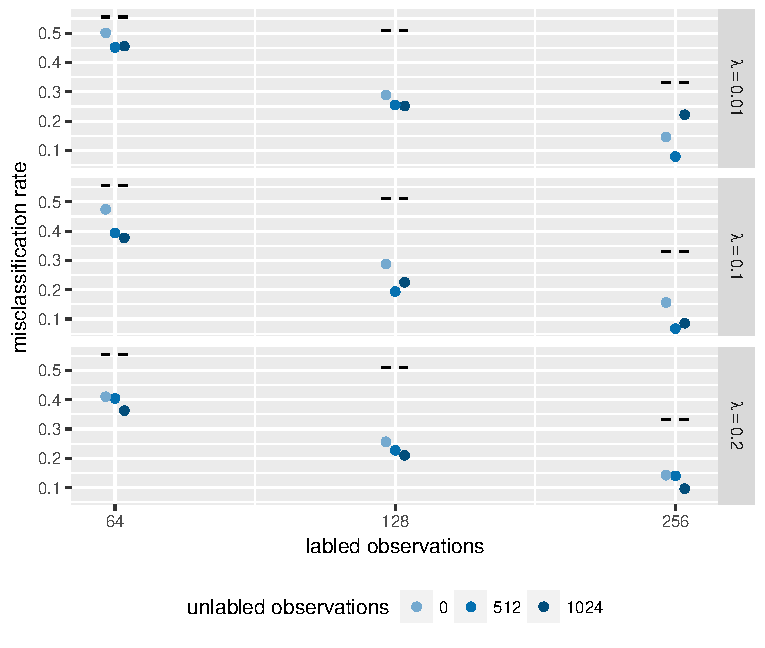
\includegraphics[scale=1]{semi-bytenet/synthetic-digits-grid.pdf}
    \caption{Shows the Semi-Supervised ByteNet model test performance depending on \textit{labeled dataset size}, \textit{unlabled dataset size}, and \textit{unlabeled learning factor}. The dashed line is a baseline that uses attention based RNN for translation on the same dataset.}
\end{figure}

\clearpage
\section{Simplified ByteNet}
